\chapter{System Architecture}
\label{chap:arch}

This chapter presents information concerning the architecture of the software
system both from the static and dynamic viewpoints. The static viewpoint focuses
on the physical architecture (hardware) required to deploy and run the
software system along with the manner in which the components that make such
software system are grouped. On the other hand, the dynamic viewpoint focuses on
the behaviour of the software system at runtime. 

The static information is presented through the \gls{Deployment View} and the
\gls{Implementation View}. The dynamic aspects of the system are presented by
means of the \gls{UI Processing View}.


\section{Deployment view}
% The aim of the \gls{Deployment View} is to describe the different processing nodes that compose
% the deployment infrastructure and how they are interconnected. A processing node
% corresponds to a piece of hardware aimed at executing either the whole software
% system or a sub-part of it.

%\usepackage{graphics} is needed for \includegraphics
\begin{figure}[H]
\begin{center}
  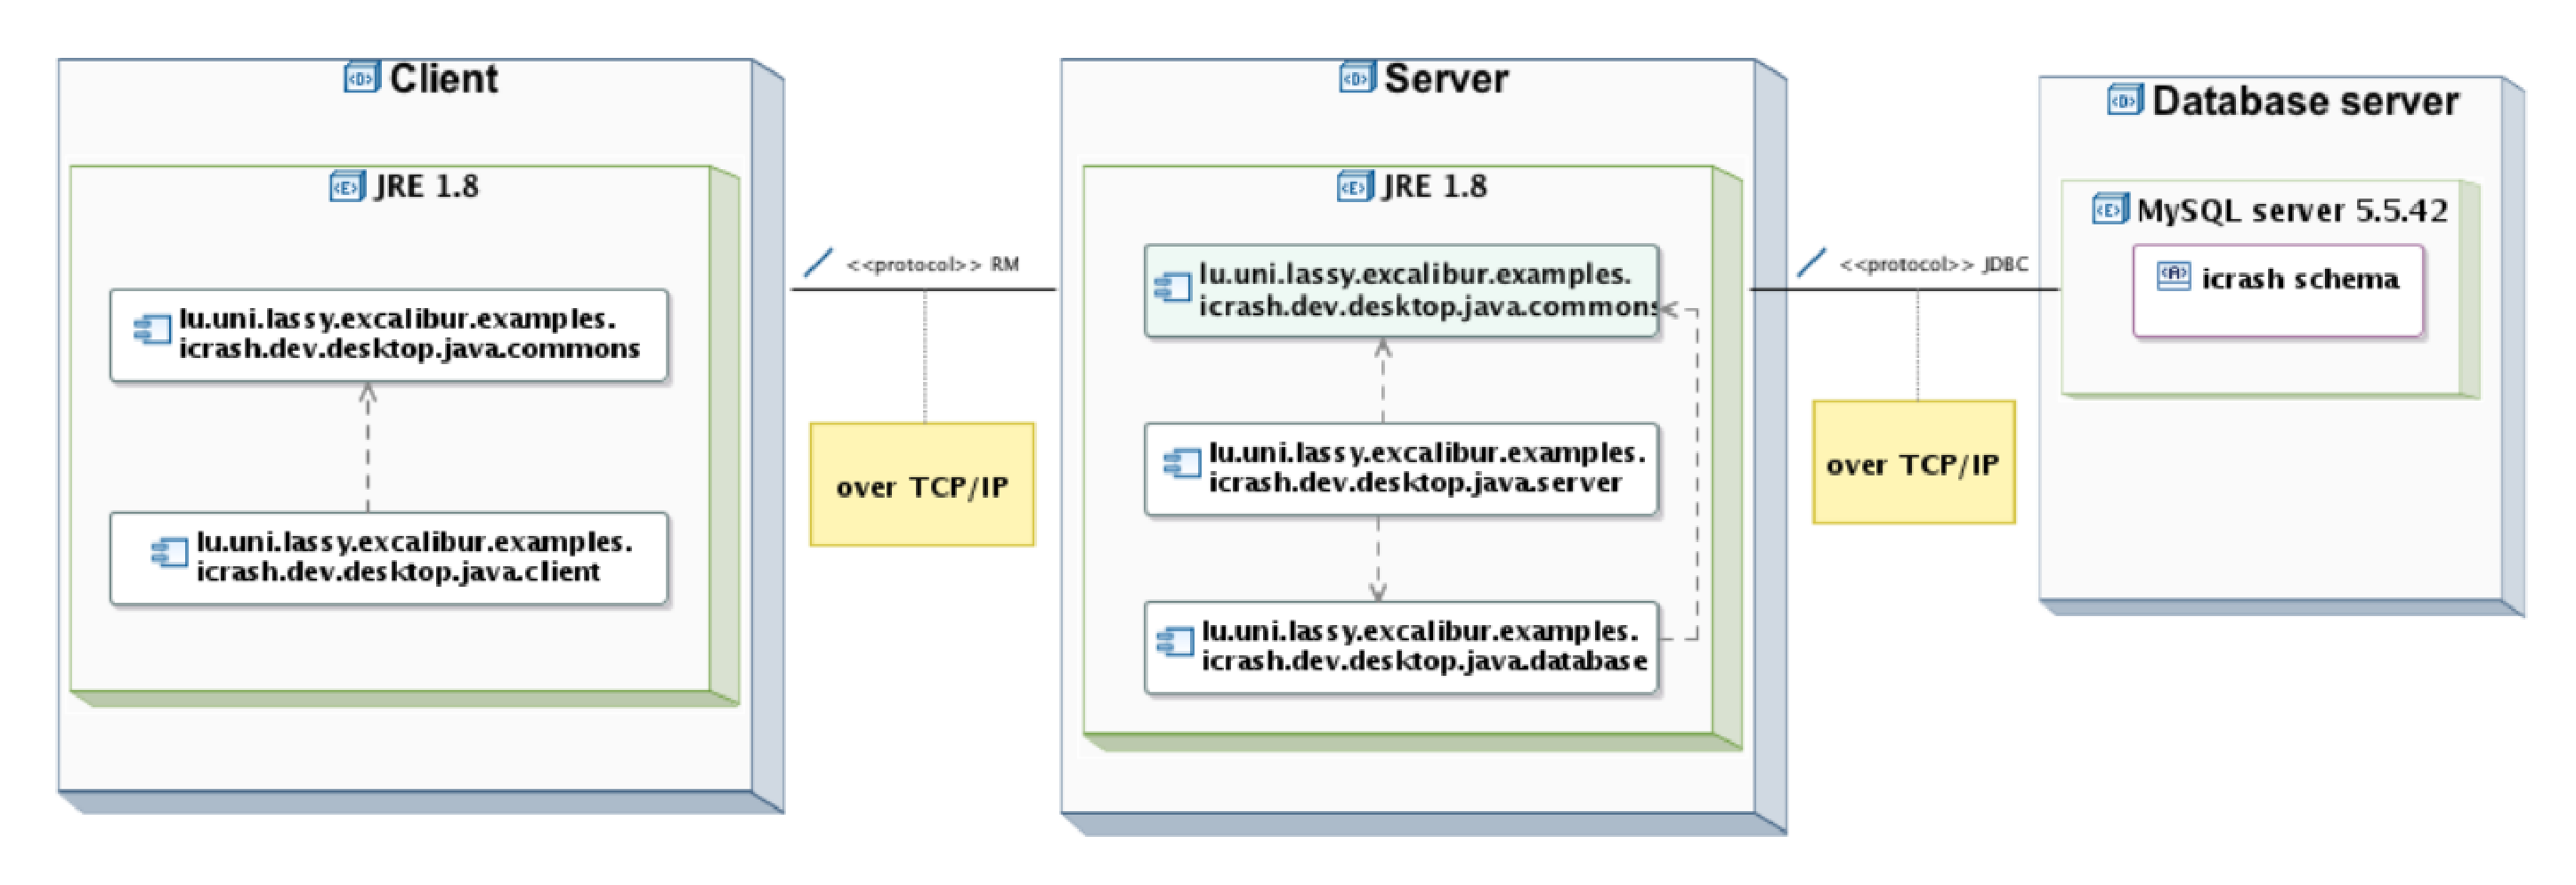
\includegraphics[width=450px]{images/architecture/deployment-view/deployment_diagram.eps}
  \caption{Deployment Diagram}
  \label{deploy-diagram}
\end{center}
\end{figure}

The system consists of 3 processing nodes:
\begin{itemize}
  \item Client node represents client's machine with launched desktop GUI
  client, whose implementation consist of two software components.
  \item Server node represents main system's machine with implementation of core
  part of the system launched. Software components include one for interaction
  with database.
  \item On database server node there is a MySQL DBMS server launched used to
  permanently store information about crises. 
\end{itemize}
 
Client and Server node interconnected using Java RMI protocol, which is built
over TCP/IP network protocol.
 
Server and Database server nodes interconnected using JDBC (Java DataBase
Connectivity) protocol, which is again works over TCP/IP.

\section{Implementation view}

%\usepackage{graphics} is needed for \includegraphics
\begin{figure}[H]
\begin{center}
  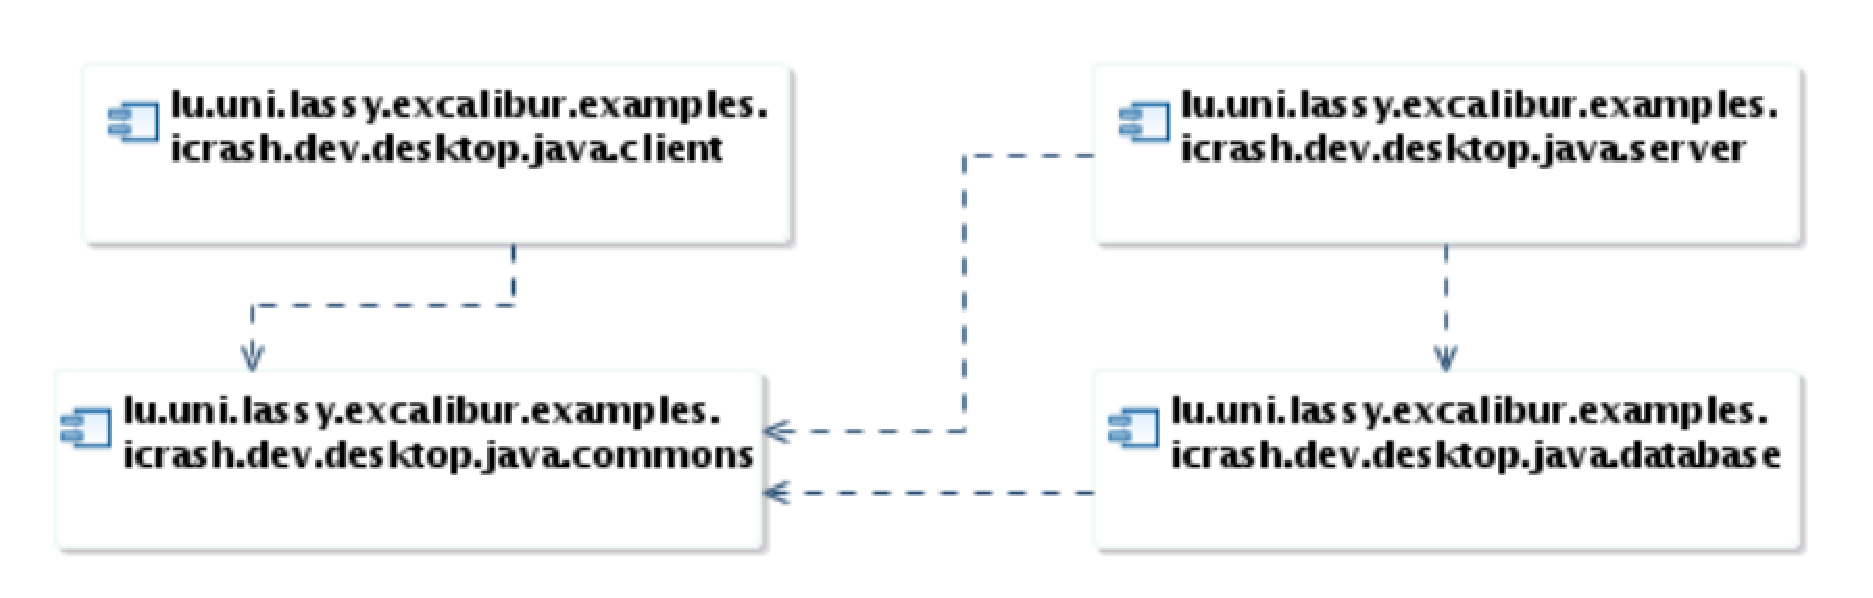
\includegraphics[width=400px]{images/architecture/implementation-view/highest_level.eps}
  \caption{High level Component diagram}
  \label{high_level_comp_diag}
\end{center}
\end{figure}

The system composed of 4 high level components:
\begin{itemize}
  \item \textbf{*.commons} consist of functionality used by all other components. It
  includes system types and some util functions.
  \item \textbf{*.client} is an implementation of desktop GUI application, used by system
  actors to interact with the system.
  \item \textbf{*.database} is used to interact with system's database server.
  \item \textbf{*.server} is an implementation of the system's core part - server which
  accepts commands from GUI client and provides system's main functionality.
\end{itemize}

\textbf{*.database} component is used by \textbf{*.server} one to performs
operation on data storage.


% The \gls{Implementation View} describes each software system component and how
% they are organised and combined to make the targeted software system.


\subsection{Component lu.uni.lassy.excalibur.examples.icrash.desktop.java.commons}
\begin{figure}[H]
\begin{center}
  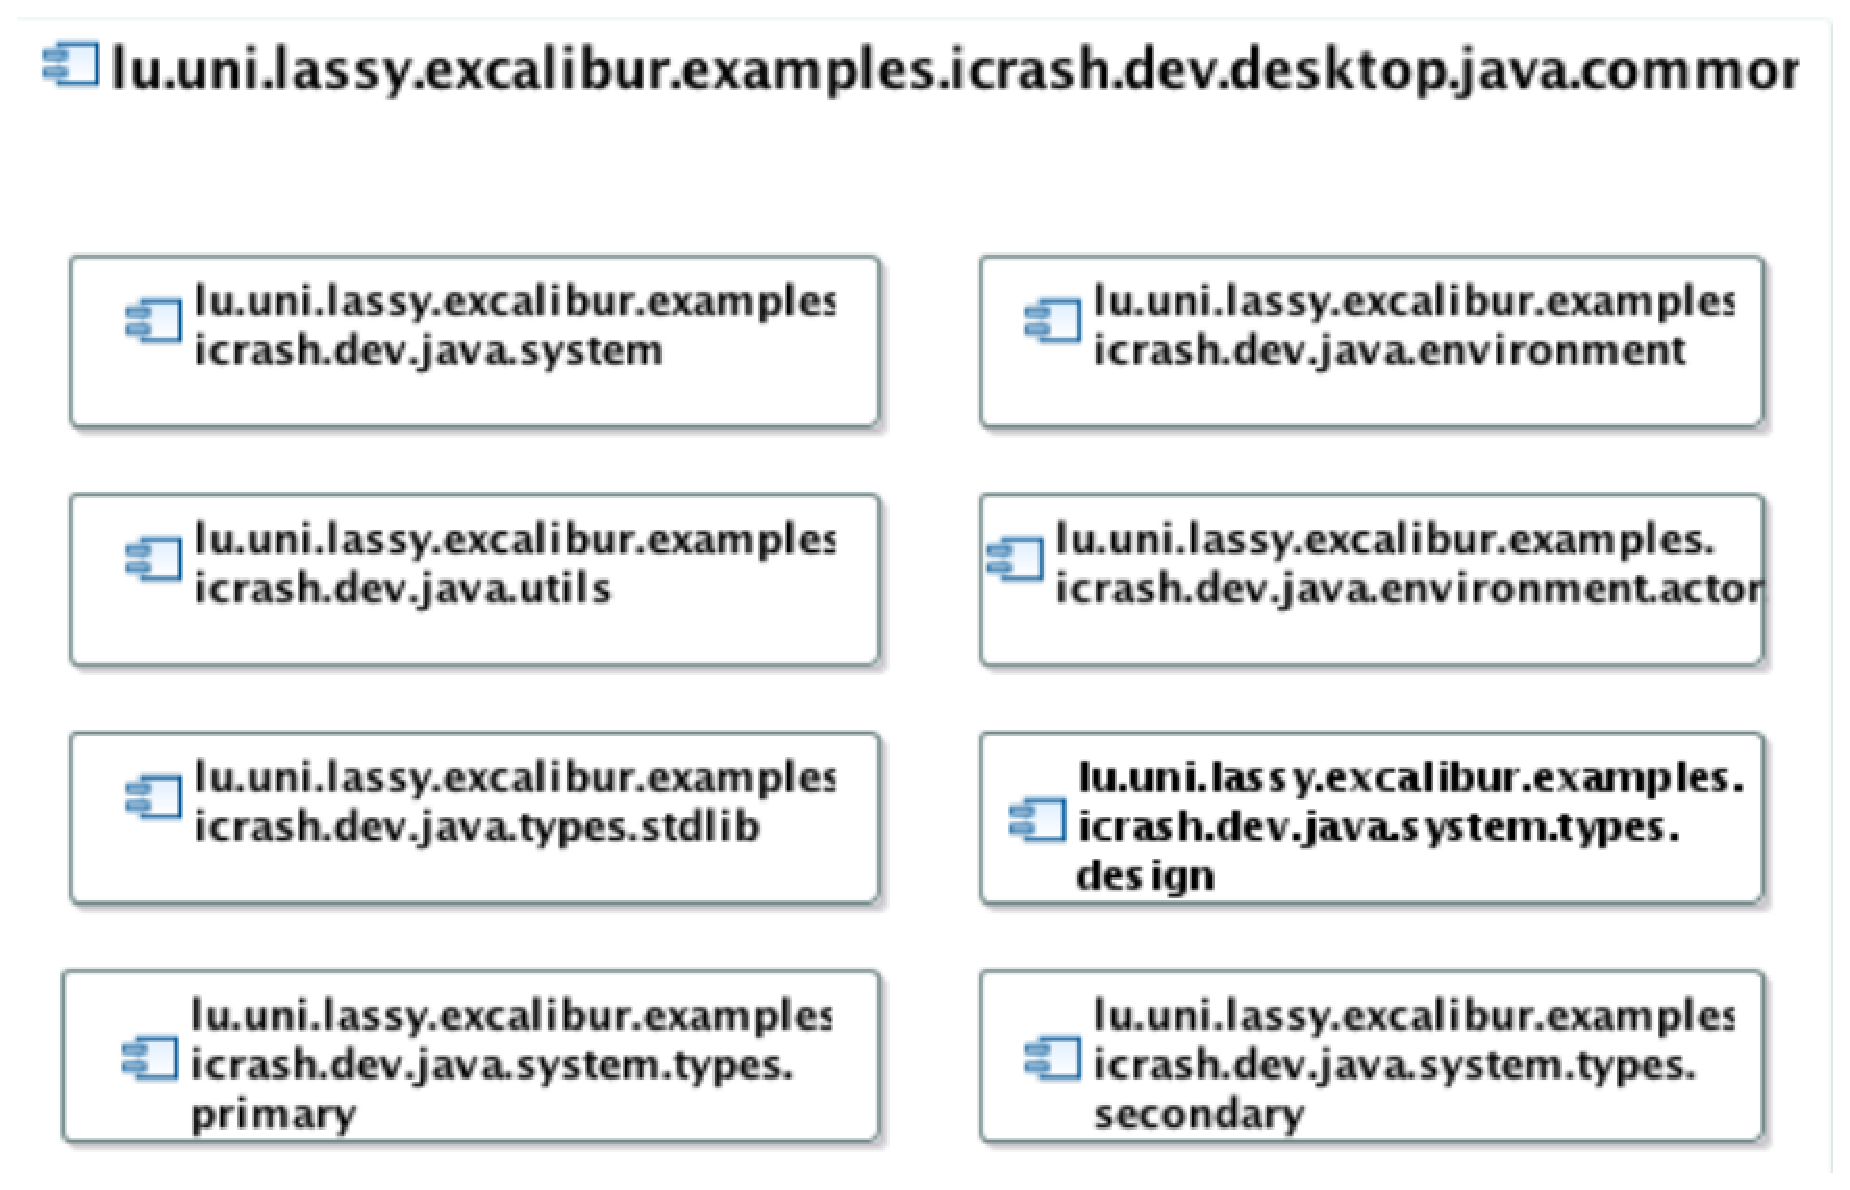
\includegraphics[width=350px]{images/architecture/implementation-view/commons_project.eps}
  \caption{Commons Project Component diagram}
  \label{commons_project_comp_diag}
\end{center}
\end{figure}

This components contains common functionality used by all other high level
components. 

\textbf{*.system.types.*} components contain system's types.

\textbf{*.types.stdlib} component includes standart library of datatypes.

\textbf{*.utils} provides some util functions.

\textbf{*.environment.actors} contains types representing system actors. 

\subsection{Component lu.uni.lassy.excalibur.examples.icrash.desktop.java.client}
\begin{figure}[H]
\begin{center}
  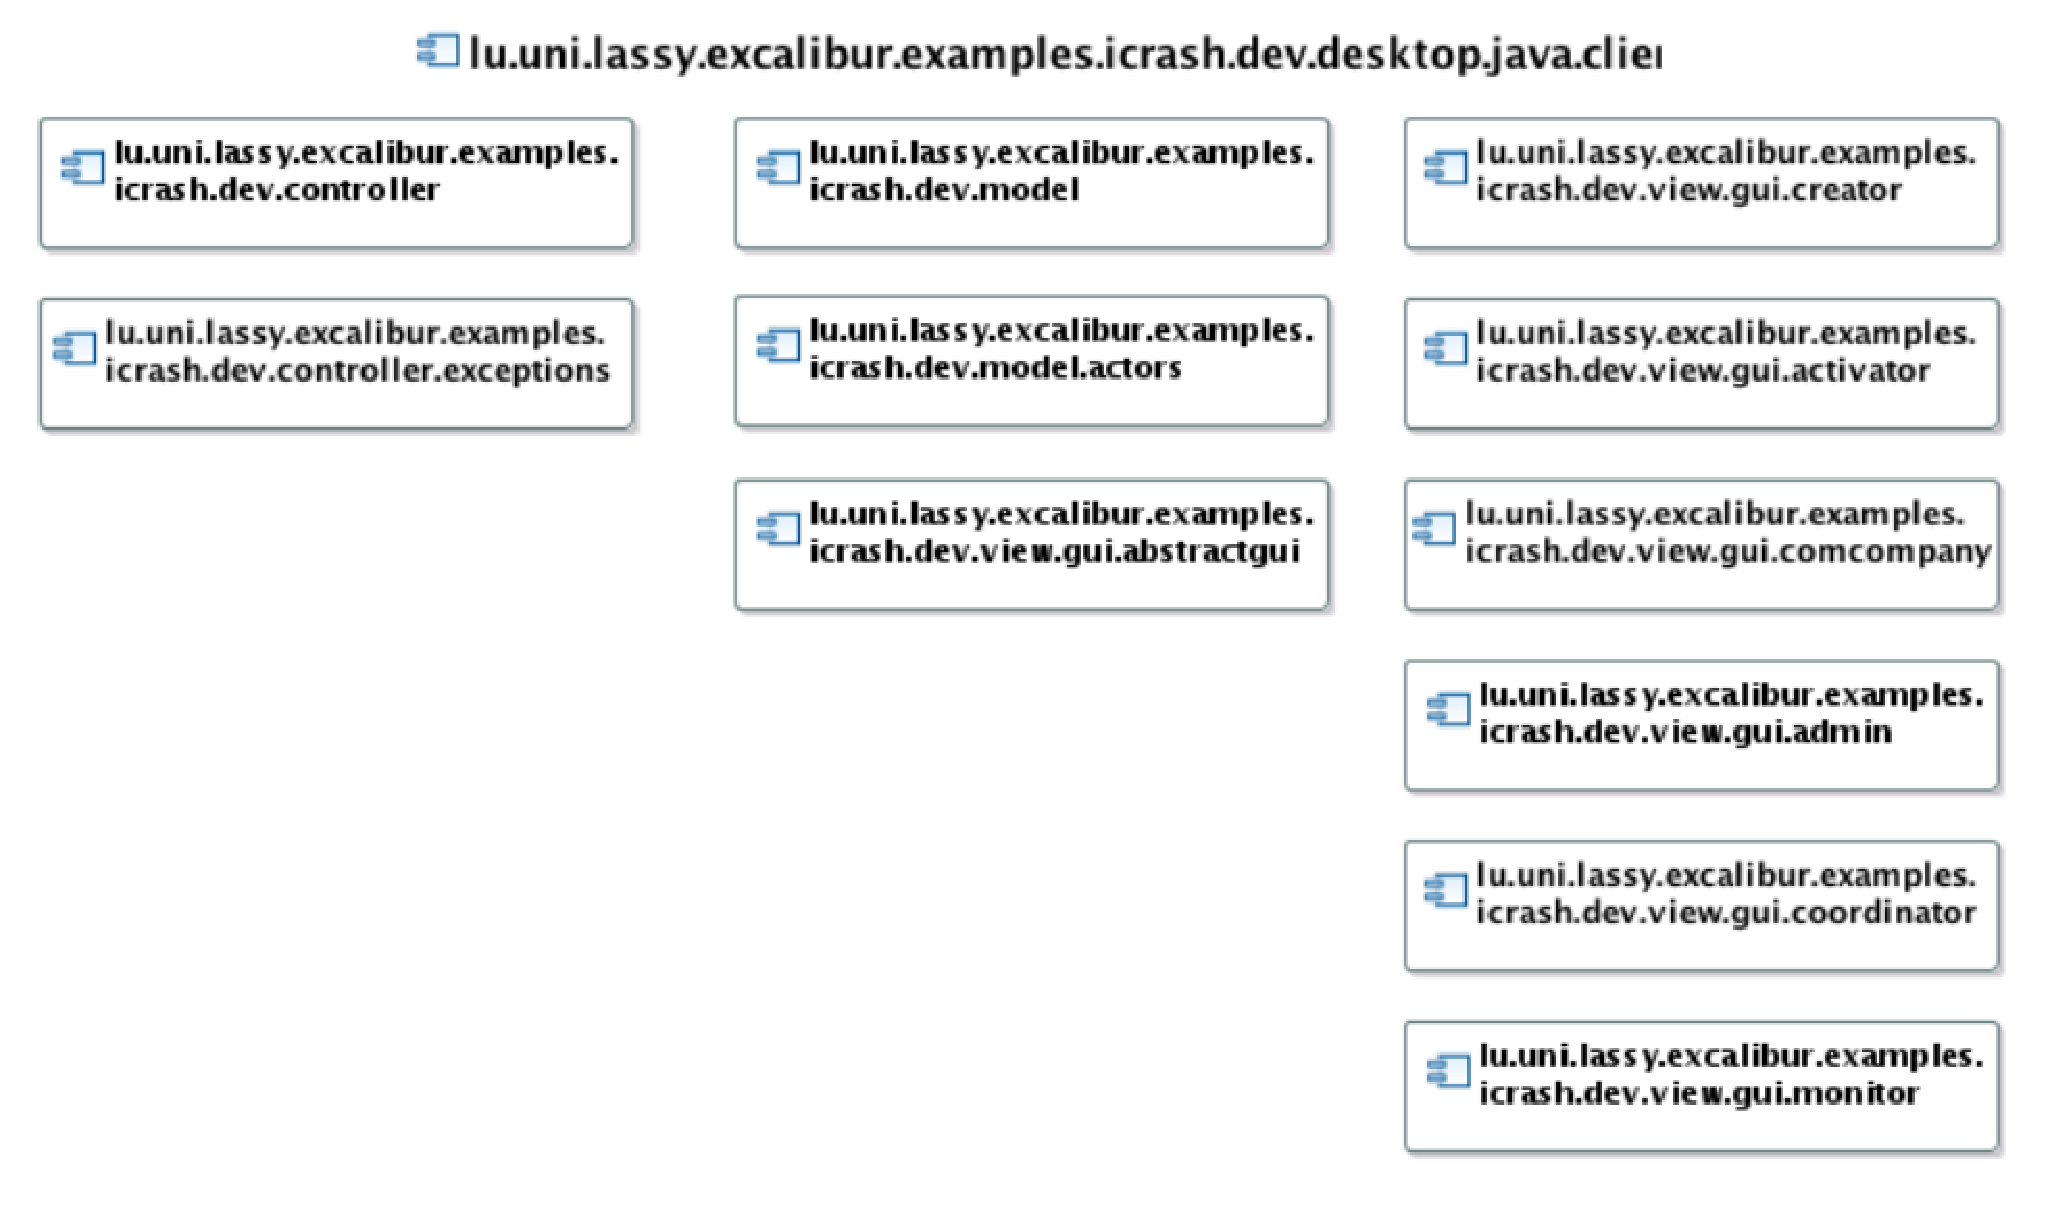
\includegraphics[width=400px]{images/architecture/implementation-view/client_project.eps}
  \caption{Client Project Component diagram}
  \label{client_project_comp_diag}
\end{center}
\end{figure}

This component contains desktop GUI application used to interact with the
system. The component is built using MVC architecture.

\textbf{*.controller.*} components contain Controller of MVC architecture, which
contain logic of business work.

\textbf{*.model.*} components represents Model part of MVC.

\textbf{*.view.gui.*} components represents View part of MVC, i.e. application's
GUI.

\subsection{Component lu.uni.lassy.excalibur.examples.icrash.desktop.java.database}
\begin{figure}[H]
\begin{center}
  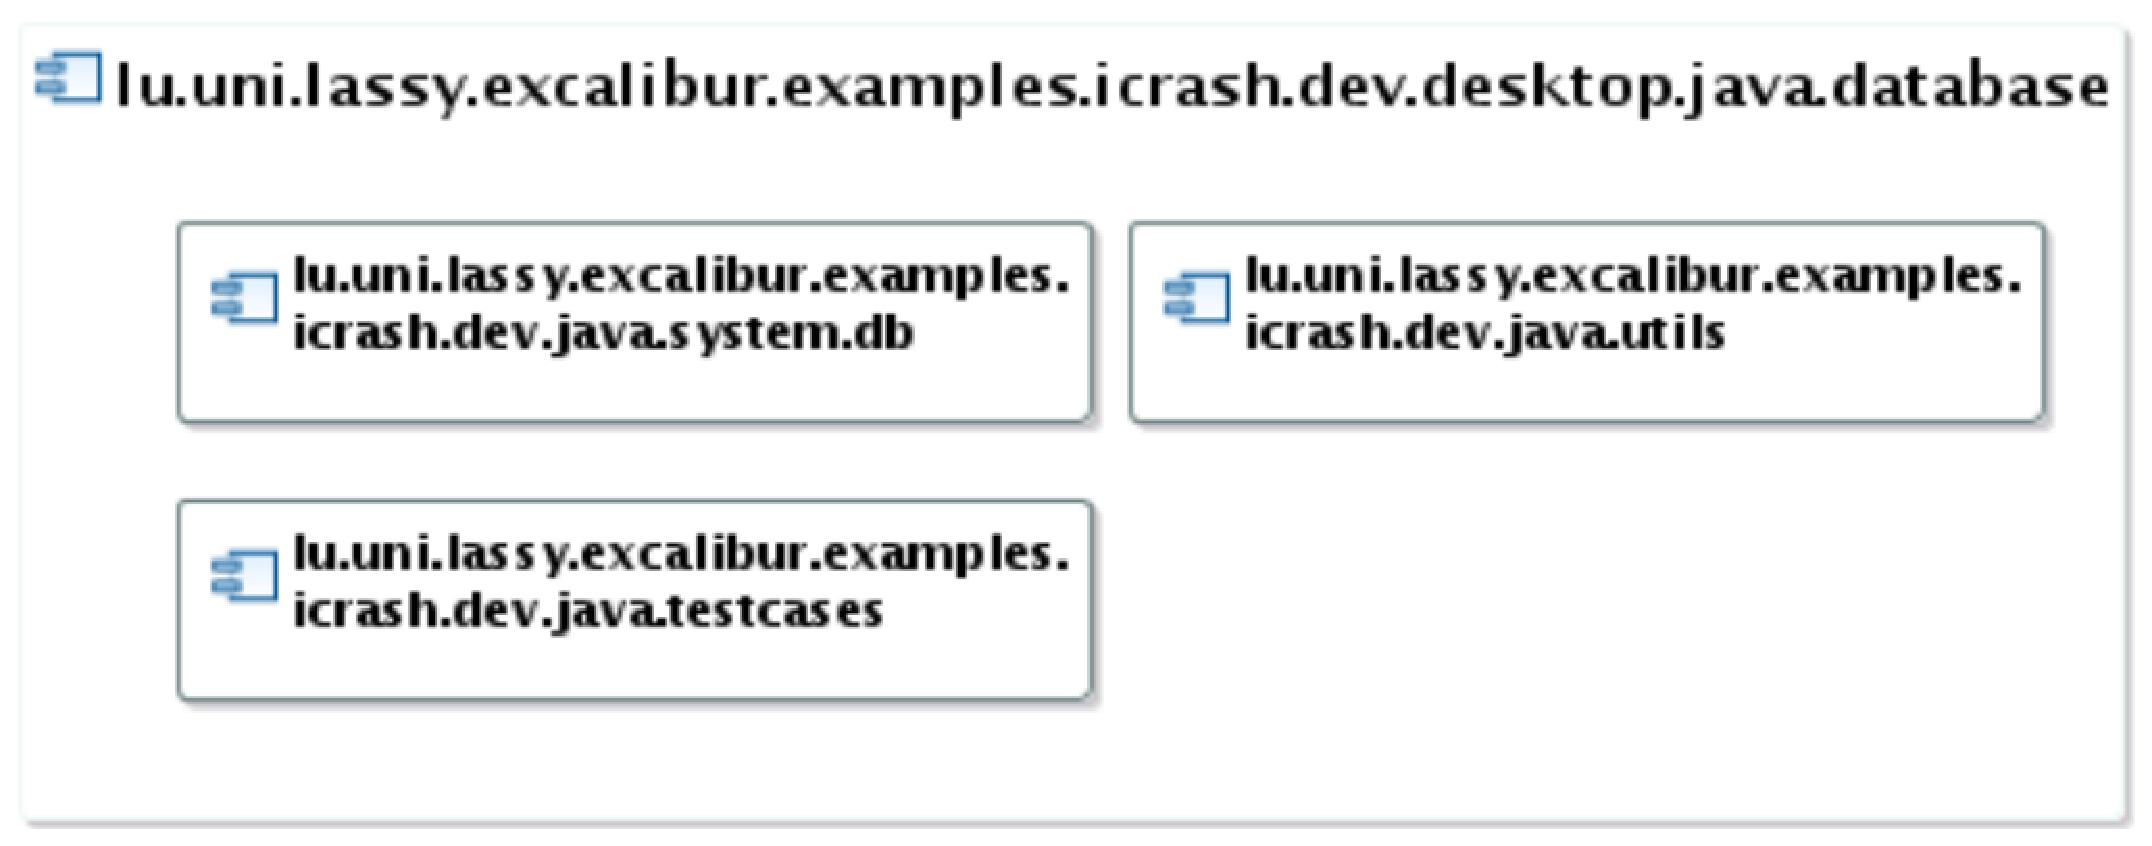
\includegraphics[width=350px]{images/architecture/implementation-view/database_project.eps}
  \caption{Database Project Component diagram}
  \label{database_project_comp_diag}
\end{center}
\end{figure}

The component allows to interact with system's data storage (database server).
E.g. add new coordinator, get existing crises, etc. 


\subsection{Component lu.uni.lassy.excalibur.examples.icrash.desktop.java.server}
\begin{figure}[H]
\begin{center}
  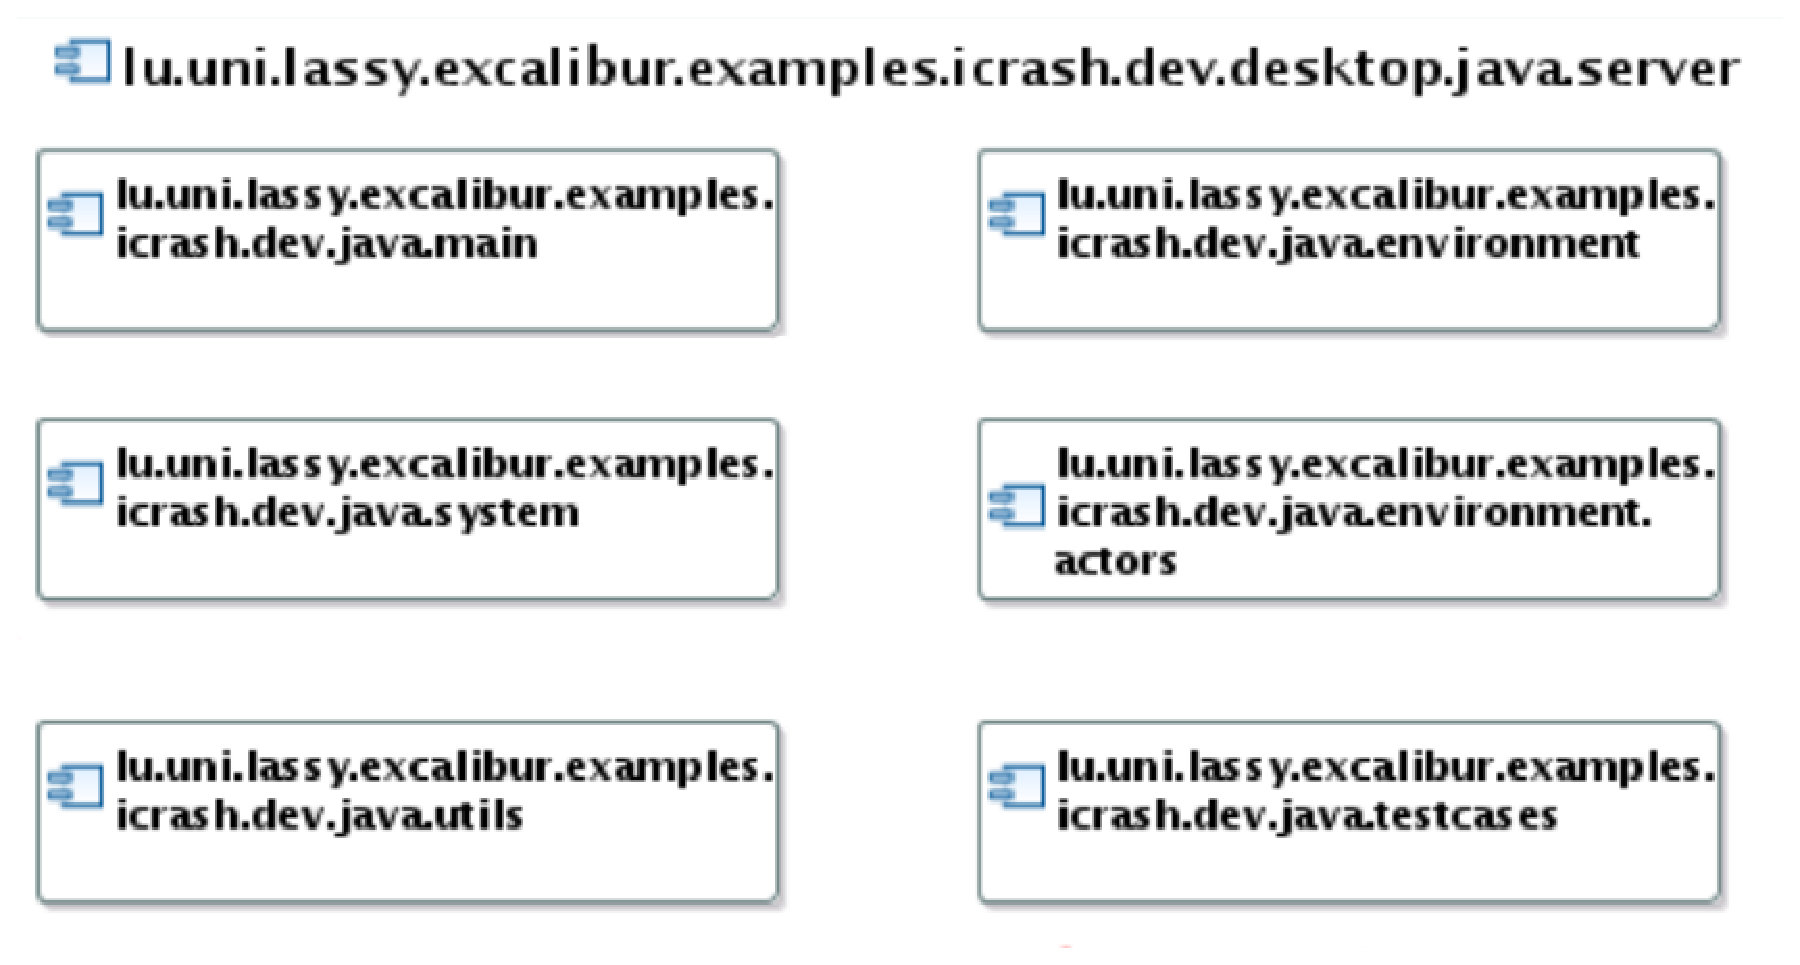
\includegraphics[width=350px]{images/architecture/implementation-view/server_project.eps}
  \caption{Server Project Component diagram}
  \label{server_project_comp_diag}
\end{center}
\end{figure}

The component represents the system's core part - server which provides system's
main functionality (handling crises) and answers to requests from GUI client.

\textbf{*.main} used to launch the server.

\textbf{*.system} contains system's main functions, built using other software
components.

\textbf{*.testcases} tests used to check server's availability.

\textbf{*.environment.*} - implementation of main system's actors
representations.


\section{UI Processing view}
A \gls{UI Processing View} is aimed at explaining the required message exchanges
to achieve the launching of a system operation (specified in the \msrmessir
Analysis Document). These required message exchanges (which are not specified in
the \msrmessir Analysis Document) make part of the user interface (UI). Thus, the
main interest of a UI Processing View is to describe the design choices made
at the UI level, such that a system operation is launched. The description
of a UI Processing View is given by means of a UML Sequence Diagram. 


A complete Design Document should contain a UI Processing View for each
non-proactive system operation specified in the \msrmessir Analysis Document, as
such kind of system operations are launched by actors through UIs that allows
them to make so. 



\subsection{UI Processing view for system operation oeSystemOperation1}
TODO

 
\subsection{UI Processing view for system operation oeSystemOperation2}
TODO


\subsection{UI Processing view for system operation oeSystemOperation3}
TODO





\section{Non-functional runtime concerns}
The description of the runtime processes should be complemented with free
textual information regarding concurrency, distribution, performance and scalability aspects.


\subsection{Performance}
TODO



\subsection{Concurrency and Parallelism}
TODO




\subsection{Scalability}
TODO






